\documentclass[12pt]{article}

\usepackage{latex/ediArticle}  %from ediArticle.sty
\usepackage{amsmath}

% Settings for the author block
\usepackage{authblk}
\usepackage{ragged2e}
%%%%%%%%%%%%%%%%%%%%%%%%%%%%%%%%%%%%%%%%%%%%%%

% left align title, authors, and affiliations
\makeatletter
\renewcommand\maketitle{\par
  \begingroup
    \flushleft
    \LARGE \setstretch{1.1} {\@title}\par
  \endgroup
  \vspace{-0.2em}
  \begin{flushleft}
    \large \setstretch{1.1} \@author
  \end{flushleft}
}
\makeatother
\renewcommand\Affilfont{\small \itshape}


\title{Reassessing the cost-effectiveness of pneumococcal conjugate vaccines in low- and middle-income countries using opportunity cost-based thresholds}
\author[1,*]{Natalie Carvalho, PhD}
\author[1,2]{Edifofon Akpan, MPH}
\author[3,4]{Fiona Russell, PhD}
\author[5]{Mark Jit, PhD}
\affil[1]{Centre for Health Policy, Melbourne School of Population and Global Health, The University of Melbourne, Australia.}
\affil[2]{Sheffield Centre for Health and Related Research, School of Medicine and Population Health, The University of Sheffield, United Kingdom.}
\affil[3]{Department of Infection and Immunity, Murdoch Children's Research Institute, Royal Children's Hospital, Australia.}
\affil[4]{Department of Paediatrics, The University of Melbourne, Australia.}
\affil[5]{Department of Infectious Disease Epidemiology, Faculty of Epidemiology and Population Health, London School of Hygiene and Tropical Medicine, United Kingdom.}
\affil[*]{Corresponding author: natalie.carvalho@unimelb.edu.au; +613 8344 3715}

\date{}


\begin{document}

% Set font size to 13pt
\fontsize{13pt}{15pt}\selectfont

\maketitle
\textit{Funding/support:}
This study was supported by the Australian government National Health and Medical Research Council (NHMRC) Centre of Research Excellence for Pneumococcal Disease Control in the Asia-Pacific.

\textit{Financial disclosure:} None reported.

\textit{Précis:} Some pneumococcal conjugate vaccine programs in low- and middle-income countries may not be considered cost-effective under recently proposed thresholds

\textit{Acknowledgments:} Samuel Grant for assistance with literature review and data extraction.

\textit{Word count:} X,XXX %(excluding abstract, references, figure legends, tables, appendices)

\textit{Number of pages:} X %Total number of pages (including figures, tables, appendices, etc) of the article

\textit{Number of figures:} 3 %Total number of figures (including figure parts [i.e., 1a, 1b, 1c = 3]) in the main article (figures in appendices should be counted separately) Maximum 6 illustrations (tables + figures)

\textit{Number of tables:} 5 %Total number of tables in the main article (tables in appendices should be counted separately)

\textit{Supplementary material:} X Pages; X Figures; X Tables


\clearpage
%%%%%%%%%%%%%%%%%%%%%%%%%%%%%%%%%%%%%%%%%%%%%%%%%%%%%%
\section*{Abstract}

\textit{Objectives:} To analyse whether the adoption of recently proposed cost-effectiveness thresholds (CETs) based on health opportunity costs, change cost-effectiveness analysis (CEA) conclusions for pneumococcal conjugate vaccine (PCV) programs in low- and middle-income countries (LMICs). 

\textit{Methods:} We conducted a systematic literature review to identify all infant PCV CEAs conducted in LMICs. CEAs that considered quality-adjusted life years, disability-adjusted life years or life years as outcome measure, were published in English, in a scientific journal, and included an incremental cost-effectiveness ratio and cost-effectiveness conclusion were included. We re-assessed cost-effectiveness conclusions using recent upper- and lower-bound CET estimates from two sources. We evaluated factors associated with evaluations that switched from being cost-effective to no longer being cost-effective.

\textit{Results:} We identified 57 studies containing 196 unique evaluations across 29 LMICs. Most studies (n=51) used a CET of 1-3x gross domestic product (GDP) per capita. Most evaluations (87\%) were found to be cost-effective (n=150) or cost-saving (n=20). Only 41\% (n=80) of evaluations remained cost-effective across all four updated CETs. Evaluations that switched were more likely to be comparisons of PCV7 versus no vaccination or PCV10 versus no vaccination, more likely to be conducted in lower-income settings, less likely to consider herd effects but more likely to consider serotype replacement, and had higher mean vaccine dose price among upper-middle income countries. Income group and vaccine dose price were the only statistically significantly factors related to evaluations that switched. 

\textit{Conclusions:} Under recently proposed CETs, reductions in vaccine dose price may be necessary to ensure cost-effectiveness of PCV programs.


\clearpage
%%%%%%%%%%%%%%%%%%%%%%%%%%%%%%%%%%%%%%%%%%%%%%%%%%%%%%
\section*{Highlights}
Authors should identify 2–3 "Highlights" that illustrate the paper's contribution to the field. 
\begin{itemize}
    \item What is already known about the topic?
    \item What does the paper add to existing knowledge?
    \item What insights does the paper provide for informing healthcare-related decision making?
\end{itemize}


\clearpage
%%%%%%%%%%%%%%%%%%%%%%%%%%%%%%%%%%%%%%%%%%%%%%%%%%%%%%
\section*{Introduction}

[Not started – outline only below]
-	Pneumococcal disease burden globally (and trend over time), 
-	Availability of effective and safe vaccines; PCVs recommended by WHO; But costly compared to most childhood vaccines 
-	Introduction/coverage of these vaccines: High use in high income and many low-income countries… trend in roll out over time. Lagging middle-income countries, those lacking Gavi/AMC eligibility.
-	PCV  introduction guided by HTA processes in many LMICs. Ex Thailand, Philippines, China. In other settings ex Pacific islands, no HTA processes available – based on donor or development partner support 

-	One component of HTA is cost-effectiveness analysis: CEA is method for weighing costs and outcomes in comparable method across interventions – provides guidance on value for money of new technologies. Results are typically presented as incremental cost-effectiveness ratios, in \$/QALY gained or \$/DALY averted. If a vaccine is found to be cost-saving, usually implemented pending other factors (budget impact, political and equity considerations, and other practical and logistical considerations including availability of vaccine, etc). Vaccines that are not cost-saving, but result in higher costs and higher health benefits, are often compared to country-specific willingness to pay thresholds, to determine whether an intervention is considered cost-effective, or good value for money.

-	Recent systematic reviews1-4 PCV is CE across (most)( LMICs (sometimes cost-saving). Cost-effectiveness is influenced by vaccine price (local acquisition), inclusion/exclusion of indirect effects (serotype replacement and herd effects), cross protection, disease burden (Incidence / mortality from IPD and pneumonia), and vaccine efficacy and coverage
-	Where are we at with willingness to pay thresholds in LMICs? Historically thresholds of 1-3 x gross domestic product (GDP) per capita have been used to assess the cost-effectiveness of vaccines and other interventions in low- and middle-income countries . Others thresholds have existed but unclear the origins of these, and what they are based on.

Newer  country-specific estimates 2-3 of cost-effectiveness thresholds (CETs) exist based on health opportunity costs are available. New approach to estimate threshold using empirical estimates of investments (supply side) or WTP (demand side). Several countries are in process of developing these thresholds (ex: Indonesia ). New estimates from \textcite{woods_country-level_2016} (based on 1 empirical estimate from a high-income setting), \textcite{ochalek_estimating_2018} (using multiple empirical data points, from LMICs), and \textcite{pichon-riviere_determining_2023} provide updated guidance on health opportunity costs in LMICs. \textcite{woods_country-level_2016} also provides these estimates for high-income countries.

-	Despite the World Health Organization and others recommending against using GDP per capita-based thresholds for judging the value for money of healthcare interventions most recent studies continue to do so4. Recent systematic review of 230 studies (713 interventions) published CEAs in LMICs: 1-3 × GDP/ capita was the most common type of threshold used (84.3\%) ; ~ A third of studies (34.2\%) using 1 to 3× GDP per capita applied a threshold at 3× GDP per capita. No study used locally developed thresholds. 79.3\% of interventions received a recommendation as “cost-effective”.
-	What do new(er) thresholds mean for previously published CEAs?  

The aim of this study is to investigate whether new country-specific estimates on cost-effectiveness thresholds (CET) based on health opportunity costs may impact on study conclusions about the cost-effectiveness of pneumococcal conjugate vaccine programs in low- and middle-income countries. A secondary aim is to investigate which study factors are influential in driving study conclusions that switch from finding PCV to be cost-effective to not cost-effective.


%%%%%%%%%%%%%%%%%%%%%%%%%%%%%%%%%%%%%%%%%%%%%%%%%%%%%%
\section*{Methods}
\subsection*{Systematic search}
We undertook a systematic literature search using similar search strings as a previous review on pneumococcal vaccination in children.\supercite{saokaew_cost_2016} We used the search strings “pneumococc* AND conjugat* AND (vaccin* OR immun*) AND “economic OR cost-effectiveness OR cost-benefit OR cost-utility OR cost-effectiveness OR cost-benefit OR cost-utility” in the title, abstract, and keyword fields of Web of Science, Scopus, PubMed, and EmBase (Ovid) from inception until 25 April 2022. The search was limited to low- and middle-income countries (LMICs) using country names and related LMIC terminology (see Appendix 1 in Supplementary Material). We also checked published systematic reviews on economic evaluation of PCV for additional studies.1-4

All identified titles and abstracts were screened by one author (EA) to remove studies that were clearly not related to the topic, were not primary research, or not focused on a LMIC. Two reviewers (EA, NC) independently screened the full text of studies remaining against seven inclusion criteria: (1) original articles containing a full economic evaluation (two evaluations, costs and consequences ),5 (2) focused on one or more LMICs, (3) evaluated PCV covering seven or more serotypes, (4) evaluated PCV in children less than 12 years, (5) used either disability-adjusted life-years (DALYs), quality-adjusted life years (QALYs) or life-years (LY), as outcome measure, (6) reported an incremental cost-effectiveness ratio (ICER) and (7) were in English. Editorials, letters, conference or meeting abstracts or proceedings, and review articles were excluded. Multi-country studies not reporting country-specific ICERs were also excluded. Evaluations of pneumococcal polysaccharide vaccine were excluded.

The following data were extracted by one reviewer (EA) into an Excel data extraction template: study characteristics (country, currency and cost year, World Bank country income group, vaccine evaluated and comparator, number and unit price of doses); methodological assumptions of cost-effectiveness analysis (perspective (societal or healthcare payer), time horizon, discount rate, and considerations of herd effects (with or without) and serotype replacement (with or without)); and study results (outcome measure, ICER for each evaluation where this was separately reported (by perspective, and by inclusion or exclusion of herd effects and by serotype replacement, where possible), inclusion of budget impact (yes or no), cost-effectiveness threshold used and conclusion on cost-effectiveness, for each evaluation ). A second reviewer (NC) double-extracted one-third of studies. Any inconsistencies were discussed resolved in consultation with both reviewers. The extracted data was compared with data from published systematic reviews1-4 to verify the extracted data on study characteristics, parameters and ICERs. 

Risk of bias was not assessed as this has been done by previously published systematic reviews2 and was not the focus of the current review.

\subsection*{Data preparation}
Countries were classified by World Bank country income group as upper middle (UM), lower middle (LM), and low (L) income. Where reported in a different currency, ICERs and vaccine dose prices were converted to United States dollars (USD) using year- and currency-specific exchange rates from the World Bank.6 Country- and year-specific GDP per capita estimates (in USD) were compiled from World Bank data and used to convert ICERs for all evaluations into a \% GDP per capita. We extracted country-specific upper- and lower-bound CETs from the Woods7 and Ochalek8 studies, in terms of \% GDP per capita, using the highest and lowest estimates from both studies. We then generated updated study conclusions (“cost-saving”, “cost-effective” or “not-cost-effective) for each evaluation according to the Woods and Ochalek CETs, by comparing the converted ICER (in \% GDP per capita) to the upper- and lower-bound CETs (in \% GDP per capita ). We generated four indicator variables to indicate whether study conclusions shifted from being “cost-effective” based on study specific threshold and conclusion, to “not cost-effective” (based on each of the four updated CET estimates: WoodsHigh, WoodsLow, OchalekHigh, OchalekLow). Studies where CETs were not explicitly stated were not included in the statistical analysis.

\subsection*{Statistical analysis}
We first summarised the key characteristics of studies and unique evaluations included in the review including distribution of CETs used and study conclusions. We then conducted a descriptive analysis of the evaluations that switched from being considered “cost-effective” by the study conclusion to “not cost-effective” (across any of the 4 CETs), by study perspective, type of comparison, income group, considerations of herd effects or serotype replacement, vaccine dose price by income group.

Next, we conducted two-sample tests of differences in vaccine dose price, country income group, perspective of analysis, and considerations of herd immunity  or serotype replacement among evaluations that switched from being cost-effective across any of the 4 CETs, compared to those that didn’t switch.

A series of probit regressions (one for each of the Woods and Ochalek upper and lower-bound CETs) were performed, with the outcome of interest the switch variables indicating whether an evaluation shifted from being considered cost-effective to not cost-effective using the updated CETs. Independent variables included in the regressions were perspective, country income group, herd immunity, and serotype replacement as categorical variables, and vaccine dose price as a continuous variable.

Analyses were performed using Microsoft Excel (Microsoft Corporation, 2023) and Stata version 17.0 SE (StataCorp 2021). 


\section*{Results}
\subsection*{Study sample and selection}
The systematic search from databases returned 863 articles. After excluding duplicates, 375 abstracts were screened and the full-text of 78 articles were evaluated. Of these, 55 articles met the inclusion criteria and were included.9-63 Two (2) additional studies64,65 were identified from the reference list of the previous systematic reviews, yielding a total of 57 studies published between 2008-2022 for data extraction (see  Figure 1 for the PRISMA flowchart). 

\subsection*{Characteristics of included studies}
Characteristics of the 57 included studies representing 196 evaluations are presented in Table 1. Of the 57 studies, 44 studies contributed to more than one evaluation  since they presented ICERs for a base case or scenario analysis for different countries, vaccine comparisons, perspectives, number of doses, or including or excluding herd effects. Most evaluations compared PCV10 (n=74 evaluations from 30 studies), PCV13 (n=61 evaluations from 28 studies) or PCV7 (n=24 evaluations from 14 studies) to no vaccination. A further 27 evaluations from 19 studies compared PCV13 to PCV10, while ten evaluations from six studies included other evaluations (PCV9 vs no vaccination, PCV13 vs PCV7, and PCV10 vs PCV7). Most evaluations considered three (53\%) or four doses (38\%). Most evaluations were conducted in upper-middle income countries (n=144 or 73\%), followed by lower-middle income (n=34) and low-income (n=18) countries. Slightly more evaluations adopted a healthcare or payer perspective (54\%) over a societal perspective (46\%). Out of the 57 unique studies, 14 included both perspectives in the base case or a scenario analysis. Herd immunity was considered in 32\% of evaluations (n=62 from 25 studies); and serotype replacement in 15\% (n=29 evaluations from 13 studies). 

\begin{table}[H]
    \centering \singlespacing \small
    \caption{Characteristics of included evaluations and unique studies}
    \begin{tabular}{|L{6cm}|R{4.5cm}|R{4cm}|}
        \hline
        \PlainInput{tables/tab_evals_studies}
    \end{tabular}
    \label{tab_evals_studies}
    \caption*{\footnotesize \textit{Notes:} Other evaluations included PCV9 vs NoVax, PCV13 vs PCV7, and PCV10 vs PCV7. \\
    IPD, invasive pneumococcal disease; PCV, pneumococcal conjugate vaccine; PCV7, 7-valent PCV; PCV10, 10-valent PCV; PCV13, 13-valent PCV. 
}
\end{table}

\begin{table}[H]
    \centering \singlespacing \small
    \caption{Characteristics of included evaluations and unique studies}
    \begin{tabular}{|L{2.8cm}|C{1.8cm}|C{1.3cm}|C{1cm}|C{1cm}|C{1cm}|C{1cm}|C{1cm}|C{1cm}|}
        \hline
        \PlainInput{tables/tab_evals_thresholds}
    \end{tabular}
    \label{tab_evals_thresholds}
    \caption*{\footnotesize \textit{Notes:} Other evaluations included PCV9 vs NoVax, PCV13 vs PCV7, and PCV10 vs PCV7. \\
    IPD, invasive pneumococcal disease; PCV, pneumococcal conjugate vaccine; PCV7, 7-valent PCV; PCV10, 10-valent PCV; PCV13, 13-valent PCV. 
}
\end{table}



\subsection*{Descriptive results}
[In progress]
Vaccine dose price and the range of dose price used in evaluations increased with increasing income level (mean (sd) \$3.94 (1.92) for L, \$14.54 (9.65) for LM, \$36.40 (33.90)  for UM income countries). 
Among evaluations with conclusions on cost-effectiveness, most (87\%) were found to be cost-effective (n=150) or cost-saving (n=20) and n=26 were not cost-effective when applying the thresholds originally used in the paper . In contrast, only 53-64\% (n=94 to 112) or 25-61\% (n=42-104) evaluations were considered cost-effective using the lower- or upper-bound opportunity cost estimates from the Ochalek 2018 or Woods 2016 studies, respectively. (Table 2)


\begin{figure}[H]
    \centering
    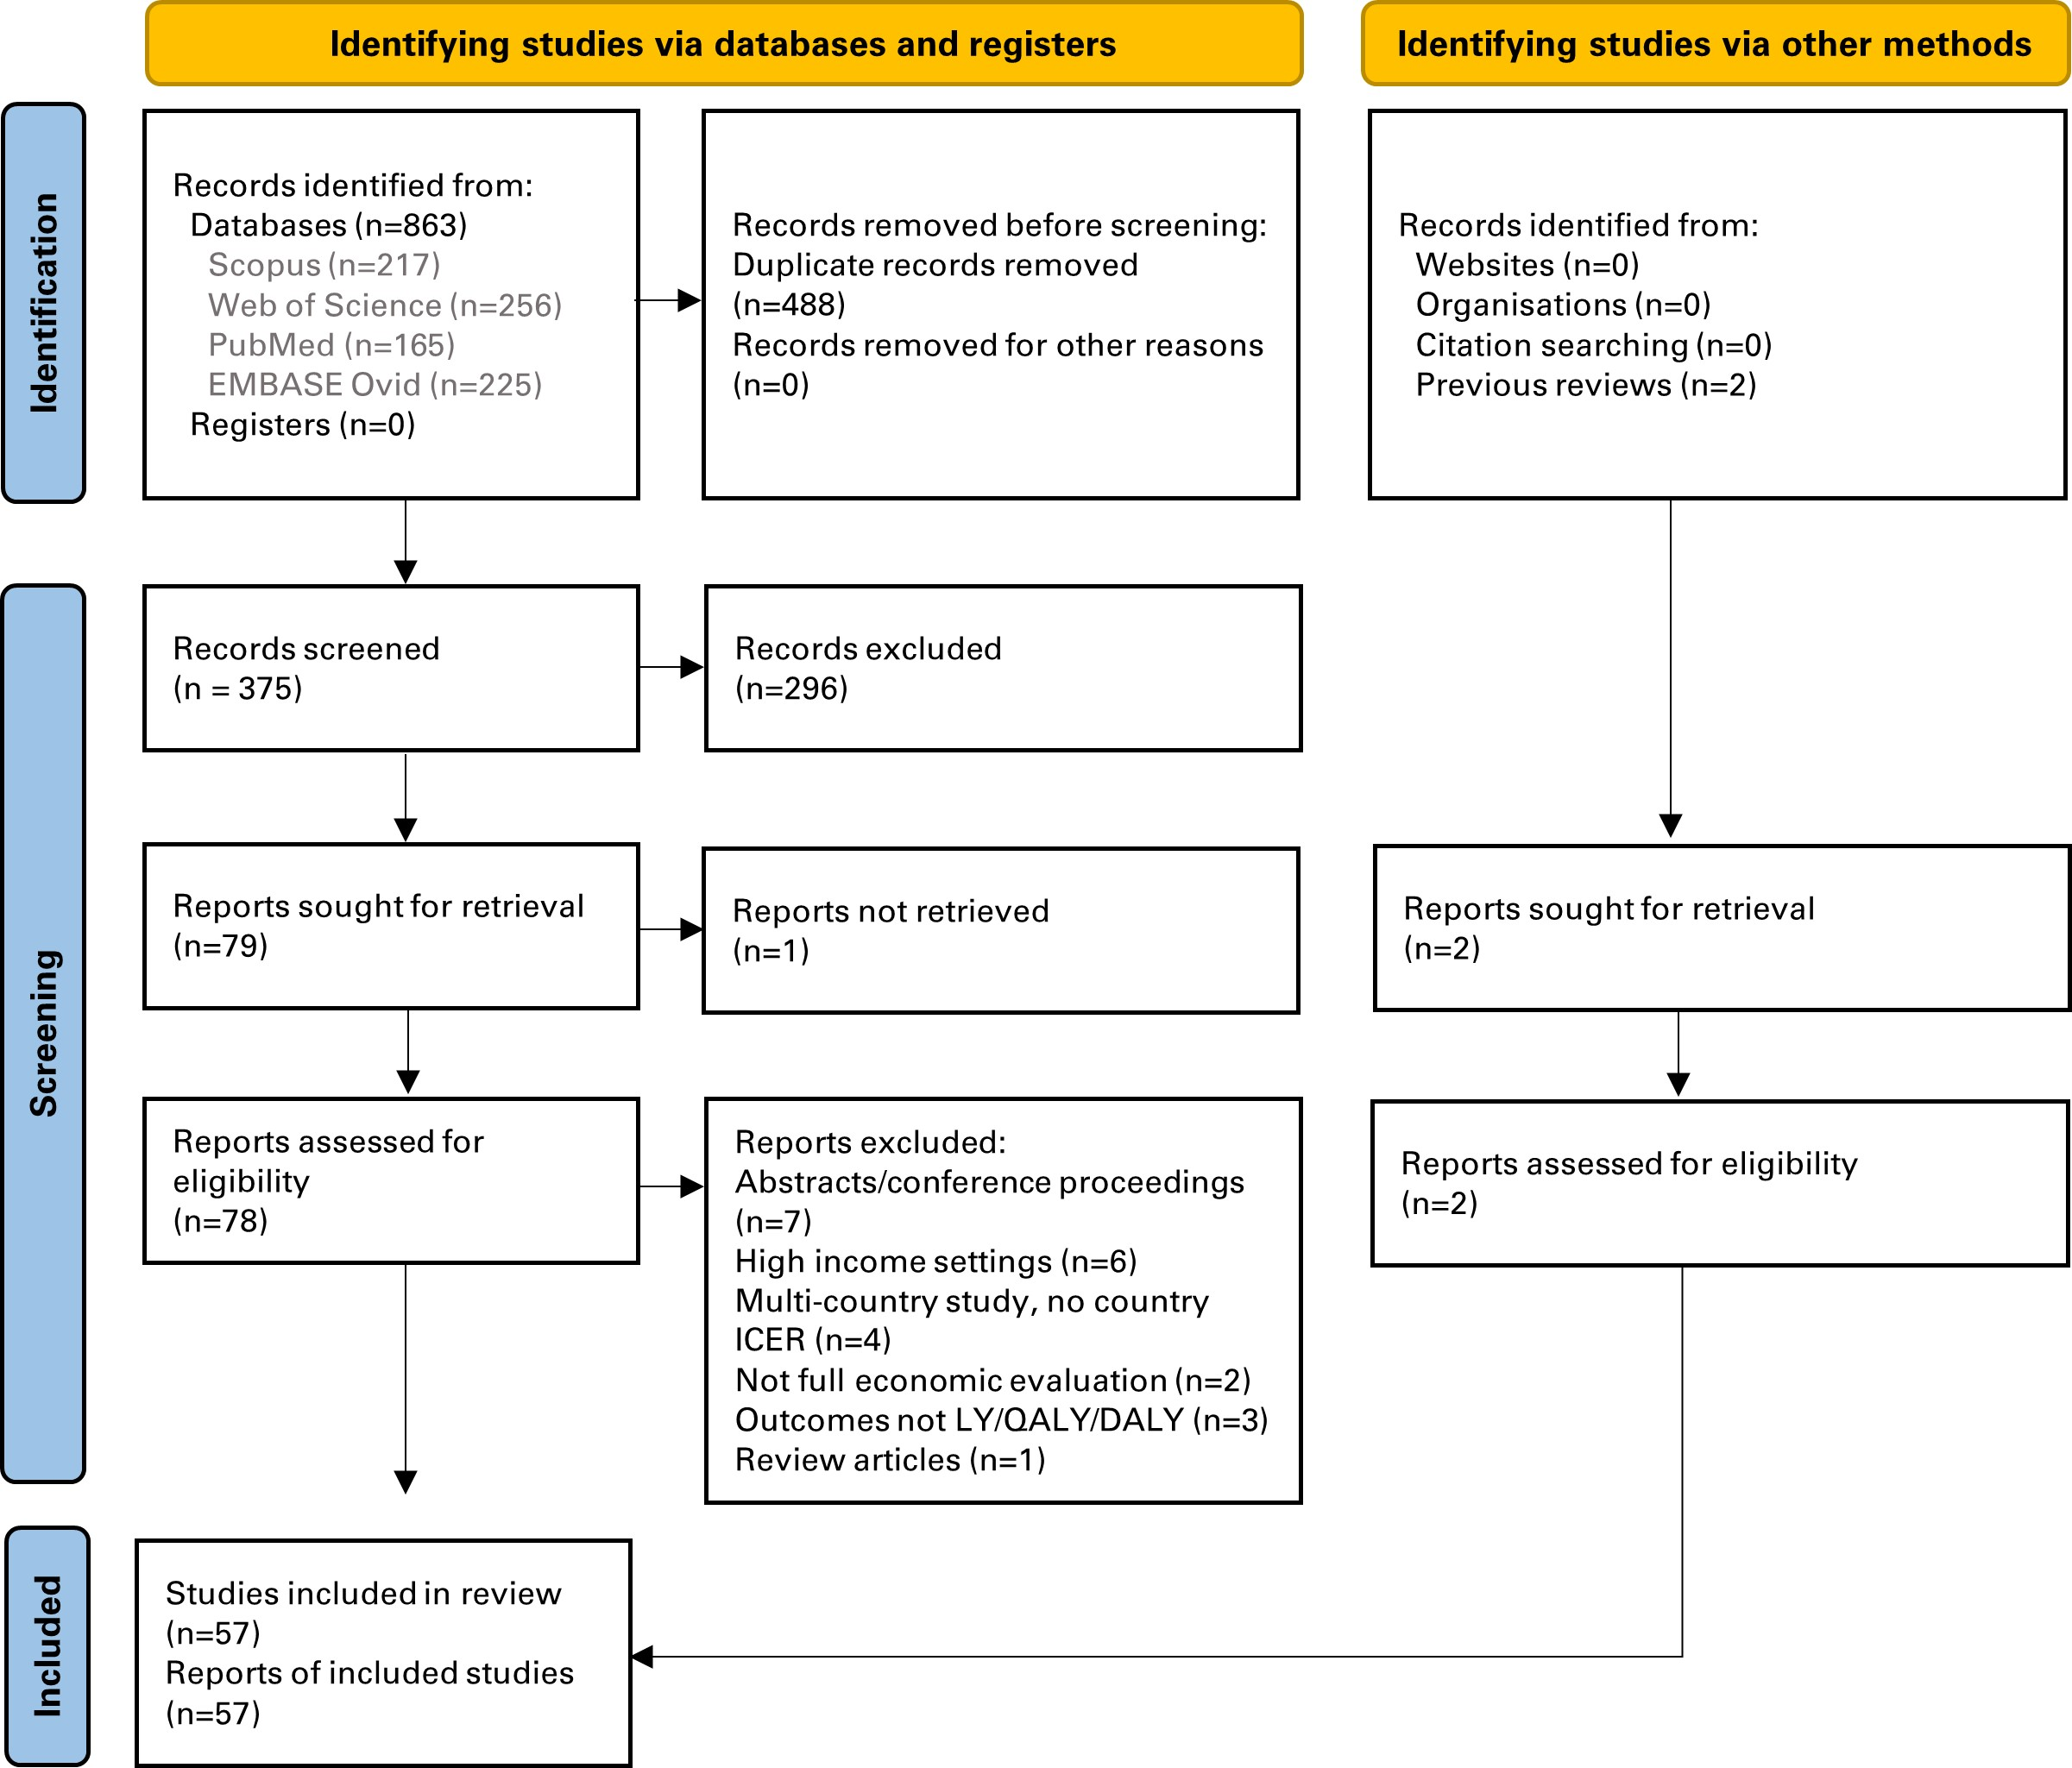
\includegraphics[width=1\linewidth]{output/figures/prisma-flow-diagram.jpg}
    \caption{PRISMA flow diagram.}
    \label{fig:prisma-flow-diagram}
    \caption*{\footnotesize \textit{}}
\end{figure}

\subsection*{Factors associated with switching from cost-effective to not cost-effective}
[In progress]
Descriptively, evaluations that switched from being cost-effective to not cost-effective under any of the updated CETs were more likely to be comparisons between PCV7 versus no vaccination or PCV10 versus no vaccination. They were also more likely to be conducted in lower income settings, not to consider herd immunity, but to consider serotype replacement . None of these associations were statistically significant according to the Pearson Chi squared test. No relationship was found between perspective of analysis and the evaluation switching from begin cost-effective. However, evaluations that switched from being cost-effective to not cost-effective across any of the new CETs had statistically higher mean vaccine dose price: \$31.82 (\$26.73-\$36.91) vs \$15.41 (\$7.26-\$23.55).  Probit regression results found vaccine dose price and country income group were the only statistically significant variables related to evaluations switching from being cost-effective to not cost-effective across any one of the updated CETs.




\begin{table}[H]
    \centering \singlespacing \small
    \caption{Characteristics of included evaluations and unique studies}
    \begin{tabular}{|L{3.5cm}|L{4cm}|L{3cm}|R{3cm}|}
        \hline
        \PlainInput{tables/tab_likely_switch}
    \end{tabular}
    \label{tab_likely_switch}
    \caption*{\footnotesize \textit{Notes:} Other evaluations included PCV9 vs NoVax, PCV13 vs PCV7, and PCV10 vs PCV7. \\
    IPD, invasive pneumococcal disease; PCV, pneumococcal conjugate vaccine; PCV7, 7-valent PCV; PCV10, 10-valent PCV; PCV13, 13-valent PCV. 
}
\end{table}




\subsection*{Sensitivity analyses}
[In progress]


\section*{Discussion}
\subsection*{Interpretation of results}
[In progress]

\subsection*{Strengths and limitation}
Multi-country studies.66-69 why don't they report at country-level – this would be useful !
[In progress by Natalie]
Strength: first paper to our knowledge to consider the impact of new, lower CETs on conclusions of cost-effectiveness across LMICs
Limitation: only considering base case ICERs, and ICERs available by differing perspective (health care payer vs societal), and with or without herd effects and/or serotype replacement.
Do not include all ICERs reported by studies (ex: through sensitivity or scenario analyses exploring different vaccine dose prices etc)

Compare results with countries that have or have not introduced PCV. Goal is not to suggest PCV should not be introduced or should be removed if not CE . But introducing a technology/vaccine when ICER exceeds WTP could be detrimental – money could be better spent on other things .
Goal – to revisit cost-effectiveness and understand whether further price negotiations are necessary . Examples of price negotiations from other settings (Indonesia? Thailand?? Ask Sarin and Itob). 

To do later:
Among low-income countries, xYZ 
Among middle-income countries – what trends do we see and does that vary by vaccine price and/or taking herd effects into account?
-	CETs are likely to vary over time, which has not been considered here
-	Further analyses to look at associations between shifts in decision-making and characteristics of evaluations.
-	Further work could link these evaluations to actual policy decisions in countries to introduce PCV (or not)
Implications for PCV Policy
[In progress]




%%%%%%%%%%%%%%%%%%%%%%%%%%%%
%%% %%%
%%% Bibliography %%%

\clearpage
\newrefcontext[sorting=nyt]
\printbibliography


\end{document}
